\documentclass{article}

% if you need to pass options to natbib, use, e.g.:
%     \PassOptionsToPackage{numbers, compress}{natbib}
% before loading neurips_2020

% ready for submission
% \usepackage{neurips_2020}

% to compile a preprint version, e.g., for submission to arXiv, add add the
% [preprint] option:
%     \usepackage[preprint]{neurips_2020}

% to compile a camera-ready version, add the [final] option, e.g.:
%     \usepackage[final]{neurips_2020}

% to avoid loading the natbib package, add option nonatbib:
     \usepackage[nonatbib]{neurips_2020}

\usepackage[utf8]{inputenc} % allow utf-8 input
\usepackage[T1]{fontenc}    % use 8-bit T1 fonts
\usepackage{hyperref}       % hyperlinks
\usepackage{url}            % simple URL typesetting
\usepackage{booktabs}       % professional-quality tables
\usepackage{amsfonts}       % blackboard math symbols
\usepackage{nicefrac}       % compact symbols for 1/2, etc.
\usepackage{microtype}      % microtypography
\usepackage{graphicx}
\usepackage{hyperref}
\hypersetup{
    colorlinks=true,
    linkcolor=blue,
    filecolor=magenta,      
    urlcolor=cyan,
}
\title{A Case Study of Deepfake Generation and Detection}

% The \author macro works with any number of authors. There are two commands
% used to separate the names and addresses of multiple authors: \And and \AND.
%
% Using \And between authors leaves it to LaTeX to determine where to break the
% lines. Using \AND forces a line break at that point. So, if LaTeX puts 3 of 4
% authors names on the first line, and the last on the second line, try using
% \AND instead of \And before the third author name.


\begin{document}

\maketitle

\begin{abstract}
Deepfakes are the most controversial application of deep learning. While they may seem to be everywhere in the media, we would like to investigate what it actually takes to build one. Our plan is to create a 5-10 second deepfake for our realistic plan. If we can go beyond that, our moonshot plan is to develop a deepfake that cannot be detected as a deepfake. We plan to build on current approaches and spend the majority of efforts on working on a neural network to create a deepfake.  
\end{abstract}

\section{Proposal}

To explore our further interests in deep learning in the year 2021, our group is looking to investigate the topic of deep fakes. We are looking to create a short deep-fake video between five to ten second long of a celebrity or other well known public figure. More precisely, we are trying to manipulate an existing clip of this individual and have them perform some actions that were not in the original video. These actions can include and are not limited to visual actions (such as mouth movements or movement of limbs) and audio manipulation (having the individual say words of our choosing in their own, natural voice. A prime example is the popular deep fake video of Former President Obama presented by Jordan Peele and Buzzfeed [12]. 

\begin{figure}[h]
\caption{Example of a Deepfake of Jordan Peele pretending to be President Obama [6]}
\centering
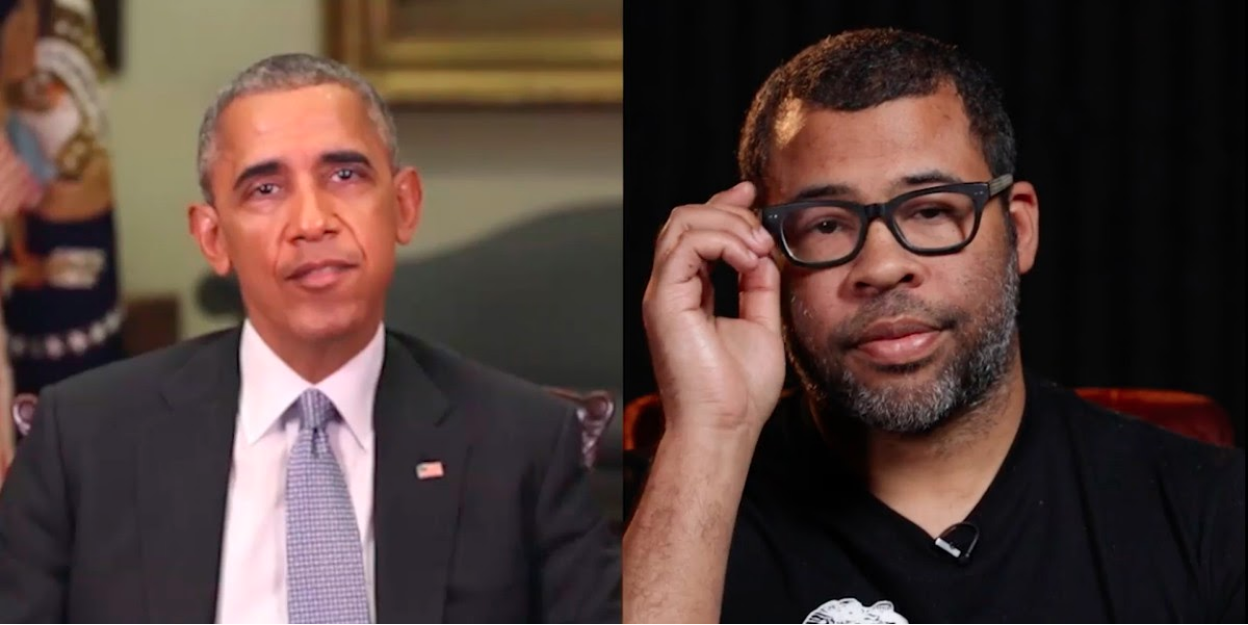
\includegraphics[width=0.9\textwidth]{Brobama.png}
\end{figure}

Although this video was produced by a numerous number of deep learning experts and visual effects artists, we are looking to see if we can recreate a smaller scale version as a group of five undergraduate students. In order to create this video, we will have to understand how to use videos with neural networks and how to use generative adversarial networks (GANs) in order to generate the fake actions of the individual. Instead of developing the deep network from scratch, we are looking to extend the findings of a deep fake paper and use their codebase as a starting point. By using already existing work, we are able to save time on development and bolster greater chances for a working final product. 



\section{Motivation}
\label{gen_inst}

In today’s state of deep learning, it is evident that deep fakes are one of the most controversial topics. There are concerns from both academia and the private sector regarding the ethics and potential dangers deep fakes can have on social, political, and economic issues. Although these concerns are valid and are growing, our group is intrigued to see how much of a threat this technology truly is for society. In other words, we are trying to see if it is feasible for a small group of undergraduate students to create a deep fake in a reasonable amount of time. 

Currently, most deep fakes are created by deep learning experts and high level academics [3]. If we are unable to develop a deep fake for large reasons, then our group will know there is a strong barrier to entry for the average individual looking to exploit this threat. On the contrary, if we are able to successfully produce a deep fake video, then we will know the threat is more prominent than originally thought. This discovery would allow us to advocate for stronger regulations against the misuse and unethical use of artificial intelligence and deep learning. Our group’s overarching goal is to evaluate the barrier to entry for an individual or organization looking to create a deep fake for malicious purposes. 


\section{Data Source and Exisiting Code}
\label{headings}

Using existing pytorch and other python libraries, we can use our experience building neural networks with pytorch to build the convolutional neural networks needed to create deepfakes. From our research, there are two types of deepfakes: one where we can swap the face of someone onto someone else, and one where we can animate a static image using a recorded video of someone else to make it look like the static image is performing the movement of the person in the video. 

For face swapping, there is an article called Subject Agnostic Face Swapping and Reenactment [8] which provides us very useful image manipulation functions that can detect faces and properly swap them after they’ve been passed through the neural network. The only data we would need for this step would be the images of two different people whose faces we would like to swap. 

\begin{figure}[h]
\caption{Example of a Deepfake Face Swap where the source face is mapped onto the target video}
\centering
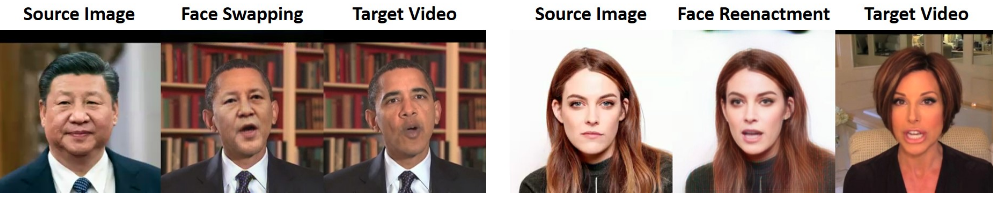
\includegraphics[width=1\textwidth]{faceswapping.png}
\end{figure}

The First Order Motion model [1] for Image Animation paper works in the same way when animating a static image based off of a video. The only data we would need is a static image of someone (preferably with a plain background) and then a video of one of us talking and moving our head. We would like to test moving our heads in different manners to see how far we can push the system to try and find some threshold that will break the deepfake. 

\begin{figure}[h]
\caption{Example of a source images being animated by a driving video}
\centering
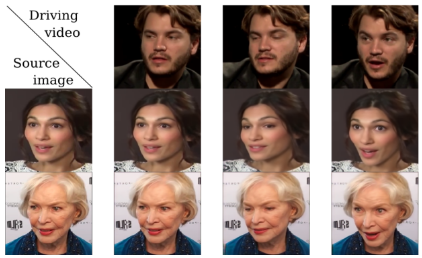
\includegraphics[width=0.9\textwidth]{animation.png}
\end{figure}

Once we are able to create these deepfakes, we would like to test how realistic we can make them and measure their realism using deepfake detection algorithms. By using the algorithms to quantize our deepfake believability, we can see for what value of believability humans are able to detect deepfakes themselves. 


\section{Baselines and Relevant Papers}
Deepfakes have generated a lot of buzz in the deep learning world recently, so there are many research papers out there on this topic. We plan to start with the models in these papers and expand on them, as we mentioned in our expected/moonshot plan above. Using the evaluation protocols we mentioned, we plan to evaluate our solution on its performance relative to other open source solutions. We will define the following as our “baselines”, as we plan to compare our solution to the following equivalents:

    \begin{enumerate}
        \item DeepFaceLab [8] - Open source software for creating deepfakes \\
        Link: \url{https://github.com/iperov/DeepFaceLab}
        \item Avatarify - Open source avatar generator \\
                Link: \url{https://github.com/alievk/avatarify-python}

    \end{enumerate}

Relevant papers are listed in our references (references 8 and 9) 

\section{Expected and Moon-Shot Plans}

For our expected achievable plan, we would like to make a short 5-10 second deepfake video. We want to achieve this because we believe that we can use existing deepfake resources and algorithms to create a semi-realistic deepfake that we can share. The main process starts with finding a video that we want to do the deepfake on, and picking a mask, or the person whose face we would like to use to put on the video, and then get the data for the mask and use neural networks to allow for the mask to be fit over the original video. The difficulty in this comes from picking the right data and making sure that the deepfake will actually be realistic with the neural network that we design. We are looking towards other neural network models for some inspiration and ideas on how we can make it as realistic as possible, which leads into the moonshot plan that we would like to develop. [4] 

Our moonshot plan is to make a deepfake so realistic that not even a deepfake detection algorithm will be able to realize that we have created a deepfake. Common deepfake detection tools rely on certain criteria to determine whether or not a deepfake is real, and some of these indicators are “changes or alterations in the colors of the face reduction in the amount of times a person will blink with their eyes, the changes in lighting that can be slightly off at some point in the video, the audio sync between the lips and the original audio of the video itself, a distinct blurriness in the area where the face will meet with the neck and / or hair.” [1] Knowing these indicators will be a big help in trying to achieve this because we know how the algorithm works and what it may be looking for, which will allow for us to try and circumvent the detection of the algorithm. 


\section{Evaluation Protocols}

For our expected plan, our aim is to at a minimum create a short deepfake video. We are interested in evaluating if this can be detected as a deepfake. It is not the aim of this realistic plan to make the most convincing deepfake but one that passes off as a deepfake. We want to create something that looks convincing but we realize that it is very unlikely that what we produce will look perfect.

We can use this website, https://sensity.ai [10], where we can upload the deepfake that we create and it will look for manipulations in the video to see if it is in fact a deep fake. This service uses several tests on videos to see if the given video is authentic or fabricated. It is also designed to find AI-based manipulation and synthesis techniques within the video. Uploading the deepfake we create here would allow us to know that what we created passes as a deepfake.

If we get to work on our moonshot plan, then we could use this tool to see if what we have created is something that cannot be detected as a deepfake. Though, that is very unlikely. 
Another idea we had for seeing if what we create is convincing is to show the deepfake that we produce to a variety of people and see if they believe that it is a deepfake or a real video. This is a much less rigorous test of “deepfake-ness” since people will not be able to look for all of the tiny details that deep fake detection algorithms look for.



\section*{Broader Impact}

\subsection{Potential Risks}
Deepfake is nothing new as it has been an area of computer graphics research since the 1990s. It was not until a new machine learning technique called Generative Adversarial Networks (GANs) appeared in 2014, providing a breakthrough in Deepfake technology. Year by year, the visual disparity between real people and these Deepfakes became indistinguishable and picked up a tremendous amount of attention after the publication of AI-manipulated pornography that featured an actress from “Wonder Woman.” As you’d imagine, this type of misrepresentation of someone would be seen as a threat to celebrities with a public image to uphold. With Deepfake in the hands of the public, the entire career of an individual could be tarnished with a leak of a false image with malicious intent. 

A darker and more grim reality of this technology could not only impact individuals but could impact nations as a whole. It is possible for someone with Deepfake technology who could potentially create a Deepfake video of a nation’s leader telling another nation’s leader that they aimed and launched nuclear weapons [2]. Out of panic and distress, the targeted nation could retaliate, which would trigger an all-out nuclear war based entirely on a world leader’s misrepresentation. Such a reality would be quite unfortunate; however, it is not entirely impossible. The power of Deepfake technology has its dire consequences and can be seen as a weapon of misformation. 

\subsection{Benefits of Deepfakes}
Though the risks of Deepfake are indeed haunting, the benefits can also be used for good in cinematography. To maintain continuity in a movie, the presence of an actor/actress who is deceased or no longer involved with the film can be generated using a combination of Deepfake and photorealistic rendering. An excellent example of this would be in Rogue One: A Star Wars Story (2016) [5], where young Carrie Fisher (actor of Princess Leia) makes an appearance at the end of the movie, which provides a segue into the original trilogy which was made in the late 1970s. The maintenance of continuity throughout the Star Wars saga provides a consistent presence of the characters and their representations and immortalizes these characters’ essence and actors, giving fans a deeper connection with the films. Deepfake helps create a more immersive environment for viewers to enjoy. 


\section*{References}

These references include a mixture of scholarly papers and news sources.
\medskip

\small
[1] Arnold. “The 5 Best Deepfake Detection Methods To Date.” Deepfake Now, Deepfake Now, 4 Sept. 2020, deepfakenow.com/best-deepfake-detection-methods/. 

[2] Agarwal, Shruti, et al. "Protecting World Leaders Against Deep Fakes." CVPR Workshops. 2019.

[3] Hwang, Tim. “Deepfakes: A Grounded Threat Assessment.” Center for Security and Emerging Technology, July 2020, pp. 1–9., doi:10.51593/20190030. 

[4] Nguyen, Thanh, and Cuong Nguyen. “Deep Learning for Deepfakes Creation and Detection: A Survey.” 2020, pp. 1–12., doi:1909.11573. 

[5] Paur, Joey. “Deepfake Tech Drastically Improves CGI Princess Leia in ROGUE ONE.” GeekTyrant, GeekTyrant, 16 June 2020, geektyrant.com/news/deepfake-tech-drastically-improves-cgi-princess-leia-in-rouge-one. 

[6] Romano, Aja. “Jordan Peele's Simulated Obama PSA Is a Double-Edged Warning against Fake News.” Vox, Vox, 18 Apr. 2018, www.vox.com/2018/4/18/17252410/jordan-peele-obama-deepfake-buzzfeed. 

[7] Rossler, Andreas, et al. “FaceForensics++: Learning to Detect Manipulated Facial Images.” 26 Aug. 2019, pp. 1–14., doi:1901.08971. 

[8] Singh, Simranjeet, et al. 2020, Using GANs to Synthesise Minimum Training Data for Deepfake Generation. https://arxiv.org/pdf/2011.05421.pdf

[9] Santha, Akhil. 2020, Deepfakes Generation Using LSTM Based Generation Using LSTM Based Generative Adversarial Networks . https://scholarworks.rit.edu/cgi/viewcontent.cgi?article=11609&context=theses

[10] “Sensity AI: The Best Deepfake Detection Tool Online.” Sensity, 5 Mar. 2021, sensity.ai/. 

[11] Siarohin, Aliaksandr, et al. “First Order Motion Model for Image Animation.” Conference on Neural Information Processing Systems, Dec. 2019. 

[12] Vaccari, Cristian, and Andrew Chadwick. “Deepfakes and Disinformation: Exploring the Impact of Synthetic Political Video on Deception, Uncertainty, and Trust in News.” Social Media + Society, vol. 6, no. 1, 19 Mar. 2020, pp. 1–13., doi:10.1177/2056305120903408. 





\end{document}